\chapter{Ausgangslage und theoretische Grundlagen}\label{ch:theoretical}


\section{Information Retrieval}

Das Ziel dieser Arbeit besteht darin, eine Schnittstelle für einen Hörenden zu erstellen, die ihm ermöglicht, einen Zusammenschnitt aus vielen verschiedenen Podcast Episoden zu erstellen, der genau zu einem Thema passt. 
Die wichtigste Aufgabe besteht also darin, die wesentlichen Abschnitte aus den Episoden herauszufinden. 
Dazu muss das System verstehen, welche Abschnitte zu verschiedenen Anfragen passen. 

Das Thema Information Retrieval (Informationsrückgewinnung) bezeichnet den Vorgang, aus einer großen Menge unsortierter Daten bestimmte Informationen wieder zu extrahieren.
Im Gegensatz zu Data-Mining werden dabei keine neuen Daten erschaffen, sondern lediglich bereits existierendes Wissen wieder zur Verfügung gestellt.
Ein bekanntes Beispiel eines Information Retrieval Algorithmus ist der PageRank Algorithmus für die Suchmaschine Google.
Suchmaschinen sind das Musterbeispiel eines Information Retrieval Systems.
Ein User gibt Stichworte ein, über die er mehr Informationen erhalten möchte und erhält daraufhin Links zu Webseiten, die diese Informationen wahrscheinlich enthalten.

In dieser Arbeit wird die Informationsrückgewinnung auf Basis der Daten von Podcasttranskripten betrieben.
Dazu werden die Techniken der Text Embeddings benutzt, um relevante Informationen zu einem bestimmten Thema aus einer großen Anzahl an Dokumenten zurückzugewinnen.



\section{Embeddings}

\subsection{Embeddings als Computersprache}

Text Embeddings sind ein Weg die menschliche Sprache für Computer verständlich zu machen. 
Die menschliche Sprache ist ein hochkomplexes Konstrukt mit einer Grammatik, die sehr viel flexibler, kreativer, vieldeutiger und komplexer ist als Maschinensprache. 
Es gibt viele kleine Bedeutungsnuancen, diese Sprache ist stark von dem allgemeinen Wissensstand der Welt geprägt und sie ändert sich im Laufe der Zeit. 
Das alles macht es für Computer sehr schwierig die menschliche Sprache zu verstehen. 
Neuere Forschung im Bereich des Natural Language Processing bietet einige Ansätze, um dieses Problem zu lösen. 
Es gibt dazu viele verschiedene Methoden, die alle darauf abzielen, Worte oder Texte in Vektoren umzuwandeln, die den Inhalt dieser Worte oder dieser Texte repräsentieren.
Diese Vektoren nennt man Embeddings.
Das Ziel dieser Embeddings besteht für unseren Zweck darin, eine Suchfunktion zu beschreiben, die auf eine Anfrage (Query) hin, passende Dokumente aus einem großen Korpus an Dokumenten liefern kann.

\subsection{Geschichte der Embeddingverfahren}

Die ersten Algorithmen mit dem Ziel, eine große Anzahl von Dokumenten durchsuchen zu können, waren Suchalgorithmen wie TD-IDF oder BM25, die in den 1970er Jahren aufkamen.
Diese versuchten Worthäufigkeiten als Anhaltspunkt zu nehmen, um Ähnlichkeiten zwischen Dokumenten zu erkennen und Suchfunktionen aufzubauen. 

Semantische Analysen begannen erst ab ca. 1990 mit der Latenten Semantischen Analyse (LSA).
Diese verwendet Eigenvektoren, um aus einer Term-Frequency Matrix versteckte (latente) Eigenschaften zu ermitteln, welche die Dokumente besser repräsentieren als die TF Matrix an sich. 
Es werden von diesen Eigenvektoren nur die wichtigsten ausgewählt, sodass jedes Dokument sehr gut als eine Linearkombination dieser Vektoren repräsentiert werden kann.
So werden nur noch die Koeffizienten dieser Vektoren gespeichert und man kann von einer Dimensionsreduktion profitieren.
Die resultierenden Koeffizienten-Vektoren sind nun nicht mehr spärlich besetzt sondern dicht und die resultierenden Eigenvektoren bilden häufig latente Themen der Dokumente ab.

Wirkliche semantische Word Embeddings erlangten erst mit der Veröffentlichung von Word2Vec (2013) eine breitere Nutzung. 
Word2Vec verwendet ein neuronales Netz, um mithilfe der benachbarten Wörter Kontextinformationen über das eigentliche Wort zu erhalten. 
Dafür gibt es die beiden Ansätze Continuous Bag of Words und Skip-Gram.
Bei dem Ansatz Continuous Bag of Words erhält das Neuronale Netz die umgebenden Wörter als Input und das Model hat die Aufgabe daraus das Zielwort zu ermitteln. 
Dieses Verfahren wird in einem Sliding Window für jedes Wort aus einem Text wiederholt. 
Für einen bestimmten Korpus aus verschiedenen Dokumenten kann dieses Modell dadurch die Beziehungen verschiedener Wörter zueinander und die Ähnlichkeit verschiedener Wörter, die oft in gleichem Kontext vorkommen, erlernen. 
Das Verfahren des Skip-Gram funktioniert ähnlich, allerdings wird dabei für jedes Wort versucht, die umliegenden Wörter zu ermitteln. 
Dieser Ansatz dauert länger im Training, hat aber den Vorteil, dass er auch seltener vorkommende Wörter gut repräsentieren kann.

Ein Jahr später wurde GloVe (Global Vectors for Word Representations) als Forschungsprojekt von der Stanford Universität vorgestellt.
GloVe verbindet Konzepte aus LSA und Word2Vec, indem es auf der Faktorisierung einer globalen Matrix beruht, aber die Distanz von Wörtern zueinander mitberücksichtigt.
Dadurch schaffte GloVe eine weitere Verbesserung der Embeddings und wird heutzutage noch unter anderem in NLP Bibliotheken wie spaCy verwendet.[englische Wikipedia referiert auf Buch aus 2018]

Im Jahre 2018 wurde der Ansatz ELMo (Embeddings from Language Model) für Word Embeddings vorgestellt.
Dieser benutzt bidirektionale Long Short Term Memory Modelle (LSTM), um daraus Embeddings zu generieren.
LSTM Modelle basieren auf Rekurrenten Neuronalen Netzen (RNN) und gehören zu den Sequenz to Sequenz Modellen. 
Sie bestehen dabei aus einem Encoder und einem Decoder.
Der Encoder codiert eine Inputsequenz, zum Beispiel ein Dokument, zu einem Embeddingvektor. 
Der Decoder dekodiert diesen Embeddingvektor wieder in eine Sequenz, z.B. eine Zusammenfassung des Dokuments. [Quelle]
Für ELMo ist dabei nur der Encoder Teil wichtig.
Dabei werden zwei Layer von Forward und Backward LSTMs eingesetzt, die für jedes Wort den Kontext vor und nach dem Wort berücksichtigen, um semantische Embeddings zu erstellen. [Quellen]

Ein halbes Jahr später wurden die Erstellung von Word und Sentence Embeddings durch BERT revolutioniert.
BERT (Bidirectional Encoder Representations from Transformers) \cite{devlin2019} ist ein auf NLP Aufgaben spezialisierter Transformer.
Das Modell wurde von Google 2019 entwickelt und war seinerzeit das beste Modell, da es in elf verschiedenen Aufgaben im Bereich des NLP State-of-the-art Ergebnisse lieferte.
Es ist auf zwei Datenbeständen, dem BooksCorpus mit 800 Millionen Wörtern und der englischen Wikipedia mit 2,5 Milliarden Wörtern trainiert worden. 
Die Aufgaben im Trainierprozess waren die Next Sentence Prediction (NSP), bei der das Modell entscheiden muss, ob zwei Sätze wahrscheinlich zusammen vorkommen und das Masked Language Modeling, bei der das Modell unkenntlich gemachte Wörter in Sätzen wiederherstellen soll.
Dadurch hat BERT sowohl auf Wortebene als auch auf Satzebene wichtige Merkmale der Sprache gelernt.
Durch die große Auswahl an verschiedenen Themen im Trainingsprozess kann das Model für viele verschiedene Sachverhalte sinnvolle semantische Embeddingvektoren erstellen.
\cite{devlin2019}


Seit der Entdeckung der Transformerarchitektur und der Entstehung von BERT entwickelt sich der Bereich der Embeddingmodelle rasant.
Täglich werden neue Modelle publiziert und im Abstand von wenigen Wochen erreichen neue Modelle State-of-the-art Performance auf populären Benchmarks wie MTEB.  


\subsection{Embeddingvektoren}

\subsubsection{Dünne Vektoren}

Embeddings können in zwei verschiedene Kategorien eingeteilt werden: dünne Vektoren und dichte Vektoren.

Dünne Vektoren, wie der TF-IDF Algorithmus und der BM25 Algorithmus, versuchen syntaktische Eigenschaften von Dokumenten zu erfassen.
Term Frequency - inverse Dokument Frequency (TF-IDF) ist ein Algorithmus, der es erlaubt, Dokumente nach Keywörtern zu durchsuchen.
Das Verfahren verwendet Worthäufigkeiten (Term-Frequency), um Dokumente, in denen ein Wort häufiger vorkommt zu bevorzugen.
Außerdem verwendet es die generelle Auftrittsrate von Wörtern (Inverse Document Frequency) um Wörtern, die seltener vorkommen, mehr Gewicht bei der Suche einzuräumen.

Daraus bildet der TF-IDF Algorithmus einen dünnbesetzten Vektor, der die Anzahl und Seltenheit jedes im Dokument vorkommenden Wortes abbildet. 
Dünnbesetzt heißt in diesem Zusammenhang, dass der Vektor viele Einträge mit dem Wert 0 besitzt. 
Das folgt aus der Bedingung, dass diese Vektoren untereinander vergleichbar sein müssen und dadurch Einträge für jedes Wort besitzen, welches im gesamten Korpus an Dokumenten vorkommt.
Jedes einzelne Dokument enthält dabei aber nur einen Bruchteil der Gesamtwörter und damit viele Nullwerte.

Best Matching 25 (BM25) ist eine Familie von Algorithmen die versuchen, den TF-IDF Algorithmus zu verbessern, indem sie die Priorisierung langer Dokumente und zu oft vorkommende Worte ausgleichen.

Außerdem kann man diese Algorithmen noch anpassen, sodass sie auch N-Gramme als Einträge der Vektoren miteinbeziehen. 
Das heißt, dass nicht nur einzelne Wörter berücksichtigt werden, sondern auch häufig zusammen vorkommende Wörter (N-Gramme) als einzelnes Token in dem Vektor abgebildet werden. 
Das bewirkt zwar, dass die Ähnlichkeit der Dokumente in der Regel besser ermittelt werden kann, vergrößert aber die Vektoren.

\subsubsection{Dichte Vektoren}

Ein relativ moderner Ansatz besteht in der Suche mithilfe von dichten Embedding Vektoren. 
Dabei wird versucht, die Semantik (also die Bedeutung) der einzelnen Segmente mathematisch mithilfe eines Vektors zu repräsentieren. 
Dieser Vektor soll dann zur Suche nach Ähnlichkeit eingesetzt werden. 
Ein Vektor, der aus dem Satz „Ich sitze auf einer Bank im Grünen“ besteht und ein Vektor mit dem Satz „Im Park steht eine alte Bank“ sollen dabei sehr ähnlich zueinander sein. 
Der Embeddingvektor des Satzes „Ich gehe in die Bank und hebe Geld ab“ aber sollte dazu wenig Ähnlichkeit aufweisen. 
Hierbei soll erkannt werden, dass sich die ersten beiden Sätze auf eine Bank zum Sitzen in der Natur beziehen und der dritte Satz ein Geldinstitut betrifft. 
Ein solch filigranes Verständnis der Bedeutung ist nicht einfach zu erreichen. 
Ein stochastischer Algorithmus würde die Unterschiede bei solchen Homonymen in den meisten Fällen nicht erkennen können. 
Stochastische Algorithmen wie z.B. TF-IDF haben auch Probleme mit Negierungen, wie zum Beispiel in „Ich habe nichts gegessen.“ und „Nichts habe ich heute gemacht außer gegessen“.

Für unsere Aufgabe ist es sinnvoll, nicht nur inhaltliche Vergleiche zu erstellen, die überprüfen, ob zwei Sätze ungefähr die gleiche Bedeutung haben, wie "Die Sonne bringt mich zum schwitzen" oder "Ich schmelze in der Hitze".
Besser wäre eine asymmetrische Ähnlichkeit, wie sie bei Frage und Antwortpaaren vorkommt.
Zum Beispiel wäre auf die Frage: "Welche Farbe hat der Himmel bei Sonnenuntergang?" ein gute Antwort: "Der Himmel hat bei Sonnenuntergang oft orange und rosa Farbtöne."  und nicht der Satz "Wie sieht der Himmel am Abend aus?"
Diese asymmetrische Ähnlichkeit ist schwerer zu ermitteln, da man normalerweise in der Antwort Informationen findet, die in der Frage nicht vorkommen.

\subsubsection{Dimensionalität von Embeddingvektoren}

Die Dimensionalität von verschiedenen Embeddings hat Einfluss auf deren Performance.
Kleinere Embeddings verbrauchen weniger Speicherplatz und lassen sich schneller untereinander vergleichen, was den Retrieval Prozess beschleunigt.
Andererseits bietet eine kleinere Dimensionalität auch weniger Möglichkeiten für die LLMs, semantische Informationen darin zu speichern.
Das heißt aber nicht, das größere Embeddingvektoren auch gleichzeitig die Semantik besser repräsentieren müssen.
Dies hängt vor allem damit zusammen, wie leistungsstark die Architektur des Modells ist und wie viele und welche Trainingsdaten zum trainieren verwendet wurden.
Das Modell "voyage-lite-02-instruct" belegt zum Beispiel auf dem Massive Text Embedding Benchmark Leaderbord mit einer Dimensionalität von 1024 den Platz 2.
Auf den Plätzen 3-5 liegen aber Embeddingmodelle mit einer Dimensionalität von 4096.


\section{Transformer Architektur}

\subsection{Sequenz to Sequenz Modelle}

Eine Transformerarchitektur ist eine der modernsten und leistungsfähigsten Architekturen, um eine Vielzahl von  NLP Aufgaben zu lösen. 
Sie bildet dabei den Nachfolger bzw. Konkurrenten zu den bis dato vorherrschenden Rekurrenten neuronalen Netzen (RNN), Gated Recurrenten Units (GRU) oder Long-Short Term Memory Systems (LSTM). 
Ähnlich wie diese Architekturen, ist auch der Transformer ein Sequenz-zu-Sequenz-Modell. 
Der Encoderteil nimmt als Eingabe eine Folge von Tokens (einen Satz, eine Audiodatei) und der Decoderteil bildet daraus eine andere Sequenz (einen Satz, eine Audiodatei). 
In diesem Abschnitt gehen wir nur auf den Encoder ein, weil er die Embeddings erstellt.

Der Unterschied von Sequenz-zu-Sequenz-Modellen zu einem gewöhnlichen feedforward neuronalen Netz besteht darin, dass die Eingabe- und Ausgabesignale auch Sequenzen mit variabler Länge sein können.
Gewöhnliche künstliche neuronale Netze haben eine feste Anzahl an Eingangs- und Ausgangsneuronen, was es ihnen nur erlaubt, Aufgaben zu lösen, bei denen die Eingangs- und Ausgangsdaten eine bestimmte Länge aufweisen.
Anwendungsfälle für künstliche neuronale Netze sind zum Beispiel Frühwarnsysteme oder Klassifikationsaufgaben (z.B. Ziffererkennung).

\subsection{RNNs, LSTMs und GRUs}

Rekurrente neuronale Netze (RNNs) stellen eine Weiterentwicklung von feedforward neuronalen Netzen dar, indem sie eine Rückkoppelung des Ausgabesignals erlauben und somit eine variable Länge an Eingabesignalen verarbeiten können.
Das Eingabesignal muss einer Sequenz entsprechen und wird dafür in Tokens zerlegt.
Jedes Token wird dabei einmal durch das RNN propagiert bis ein Ausgabeembedding für dieses Token produziert wurde.
Das Ausgabeembedding aus der vorherigen Iteration wird dann zusammen mit dem nächsten Token in der Sequenz als Eingabe für die nächste Iteration verwendet.
Dadurch wird die gesamte Sequenz nacheinander in diesem Netz verarbeitet, wobei jedes Token den Kontext der vorherigen Tokens als Embedding mitgeliefert bekommt.
Am Ende liefert ein RNN dann ein einziges Embedding, welches die gesamten Informationen der Sequenz repräsentieren soll.

Ein Problem, welches diese Architekturen besitzen, ist das Problem des Vanishing Gradient.
RNNs versuchen immer im Encoder die gesamte Inputsequenz von links nach rechts (forward) oder von rechts nach links (backward) zu verarbeiten, um daraus ein einzelnes Embedding zu erstellen.
Informationen, die in der Mitte der Sequenz vorkommen, werden wahrscheinlich von danach folgenden Informationen überschrieben, weil das Modell versucht, alle Informationen in derselben Matrix zu speichern. 

Die Ansätze des Long-Short Term Memory System (LSTM) und der Gated Recurrenten Unit (GRU) versuchen dieses Problem zu lösen, indem sie Gates einsetzen.
Diese Gates bestimmen, welche Informationen aus dem vorherigen Embedding durch das Embedding der nächsten Iteration überschrieben werden dürfen.
Dadurch können sie wichtige Informationen länger speichern.
Bei einem LSTM werden dafür drei verschiedene Gates benutzt: das Forget Gate, das Input Gate und das Output Gate.
Jedes dieser Gates hat wiederum eine bestimmte Anzahl an Parametern, die bestimmen welche Informationen vergessen, welche für den Input der nächsten Iteration benutzt und welche bei der nächsten Iteration ausgegeben werden.
Alle diese Parameter müssen beim Training des LSTMs mittrainiert werden, was zu einem komplizierten Model und zu einem langsamen Trainingsprozess führt.
Bei GRUs gibt es nur ein Gate: das Update Gate.
Sie haben dadurch weniger Parameter, die trainiert werden müssen und vereinfachen damit den Trainingsprozess.
\cite{pirani2022}

\subsection{Transformer Encoder}

Der größte Unterschied der Transformerarchitektur zu RNNs, GRUs und LSTMs ist der Attention Mechanismus.
RNNs, GRUs und LSTMs sind darauf angewiesen, den Input sequentiell Token für Token zu verarbeiten, da jede Zelle als Input das Embedding der vorausgehenden Zelle benötigt.
Das macht das Training eines Models sehr zeitaufwendig.

Der große Vorteil der Transformer ist, dass sie parallelisierbar sind.
Alle Tokens einer Inputsequenz können synchron verarbeitet werden. 
Dabei wird für jedes Token zunächst durch ein vorher ermitteltes Word Embedding ersetzt.
Der Mechanismus des Positional Encodings stellt sicher, dass das Modell die Reihenfolge der Token mitberücksichtigen kann.
Dieser Mechanismus berechnet aufgrund der Position des Tokens in der Sequenz ein Positional Embedding auf der Grundlage von Sinus- und Cosinusfunktionen und addiert es mit dem vorherigen Word Embedding.
Das resultierende Embedding enthält damit sowohl Informationen über das Token selbst durch das Token Embedding und über die Position in der Sequenz durch das Positional Encoding.


\subsection{Multihead Self Attention}

Transformer setzen Multihead Self Attention ein. 
Der positional encoded Input wird von mehreren self Attention Köpfen verarbeitet, der sogenannten Multihead Self Attention. 
Jeder dieser Köpfe spaltet den Input in Query, Key und Value Matrix auf, indem es die ursprüngliche Embeddingmatrix jeweils mit einer vortrainierten Query-, Key- und Valuematrix multipliziert.
Die resultierenden Matrizen werden dann mithilfe folgender Formel zur Attention Matrix umgewandelt:

$Attention(Q,K,V)=softmax(\frac{QK^t}{\sqrt{d_k}})*V$

Der Parameter d stellt dabei die Dimension der Matrix k dar.

Um die Formel besser zu verstehen, wird an einem Beispiel demonstriert, was die einzelnen Matrizen für Aufgaben besitzen.
Als Eingabe wird der Satz: "Alice fuhr gestern durch die Nürnberger Innenstadt" benutzt.
Die Query Matrix beschreibt nun eine Frage an diesen Satz, zum Beispiel "Wer?".
Wie genau diese Fragen aussehen, ist nicht leicht zu ermitteln und wird nur in seltenen Fällen so ausfallen, wie auch Menschen nach bestimmten Informationen fragen.
Wichtig ist jedoch, dass in jedem Attention Kopf eine bestimmte Frage gestellt wird.
Die Key Matrix hat nun die Antwort darauf, wo diese Informationen im Satz stehen könnten, also wahrscheinlich im ersten Wort. 
Die beiden Matrizen werden nun multipliziert, um die Position der Antwort auf die Frage zu erhalten. 
Das Ergebnis wird durch Division mit der Dimension der Matrix skaliert und anschließender Softmax-Funkion normiert, um die Relevanz der Schlüssel anzupassen.
Anschließend wird die angepasste Fragen-Schlüssel Matrix mit der Value Matrix multipliziert, welche die Informationen der Sequenz beinhaltet. 
Die resultierende Matrix würde dann die Information beinhalten, dass die Antwort auf die Frage "Wer?" für den Satz "Alice fuhr gestern durch die Nürnberger Innenstadt" wahrscheinlich "Alice" ist.

Die verschiedenen Köpfe der Multihead Self-Attention liefern nun verschiedene Antworten auf verschiedene Fragen und versuchen damit die Informationen der Sequenz zu codieren.
Im Anschluss werden die verschiedenen Matrizen konkateniert und in einem weiteren feedforward neuronalen Netz in Ihrer Dimensionalität reduziert.
Die finale Embeddingmatrix kann für verschiedene Funktionalitäten eingesetzt werden.

Die Transformerarchitektur benutzt dieses Embedding, um damit im Decoder wieder neue Tokens zu erstellen.
Dafür wird eine ähnliche Vorgehensweise wie im Encoder betrieben.
Der größte Unterschied zwischen dem Encoder und dem Decoder ist, dass der Encoder den Input nur ein einziges Mal verarbeitet und die daraus entstandene Embeddingmatrix nicht mehr neu berechnet werden muss.
Dadurch ist dieser Schritt sehr schnell.
Im Gegensatz dazu wird die Decoderphase für jedes einzelne Outputtoken neu durchlaufen.
Zunächst wird dabei wieder eine Self-Attention Matrix über den gesamten bisherigen Ausgabetokens generiert.
Die Self-Attention Matrix wird dann genutzt, um eine weitere Attention Matrix zu errechnen.
Diese benötigt nun wieder eine seperate Query-, Key- und Valuematrix.
Im Vergleich zur Self-Attention werden dabei aber nicht alle Matrizen aus derselben Embeddingmatrix errechnet.
Nur die Querymatrix wird aus der vorher generierten Self-Attention Matrix generiert.
Die Key- und die Valuematrix werden aus der Embedding Matrix des Encoders berechnet. 
Dadurch wird die Information aus dem Userprompt bei der Generierung jedes einzelnen Tokens mitberücksichtigt. 
Die resultierenden Matrizen aller Attentionköpfe werden wieder durch Feedforward Netze propagiert, um sie zusammenzuführen und die Dimensionalität anzupassen.
Am Ende wird die ganze Matrix durch eine Softmax Funktion geleitet, die dann die Ausgabewahrscheinlichkeiten für alle Token generiert.
Das heißt die Ausgabe ist ein Vektor, der als Dimensionalität die Länge des Vokabulars der Token besitzt.
Welches Token am Ende generiert wird, kann zum Beispiel mit einem Greedy-Algorithmus bestimmt werden, der immer das Wort mit der größten Wahrscheinlichkeit auswählt.
Andere Auswahlmöglichkeiten wären zum Beispiel mit einem Beam-Search Algorithmus möglich, bei dem mehrere Sequenzen generiert werden, um erst später zu schauen, welche Sequenz insgesamt die höchste Wahrscheinlichkeit besitzt.
In dieser Phase kann auch eine Zufallsvaiable eingeführt werden, die immer ein Token aus den wahrscheinlichsten Token auswählt, um bei mehrfacher Wiederholung eines Prompts verschiedene Ergebnisse zu liefern.

Um bei dem Beispiel von oben zu bleiben, würde der Decoder zum Beispiel versuchen, den Satz zu vollenden mit  "Alice fuhr gestern durch die Nürnberger Innenstadt und bewunderte die beeindruckenden mittelalterlichen Bauwerke."
\cite{vaswani2023}

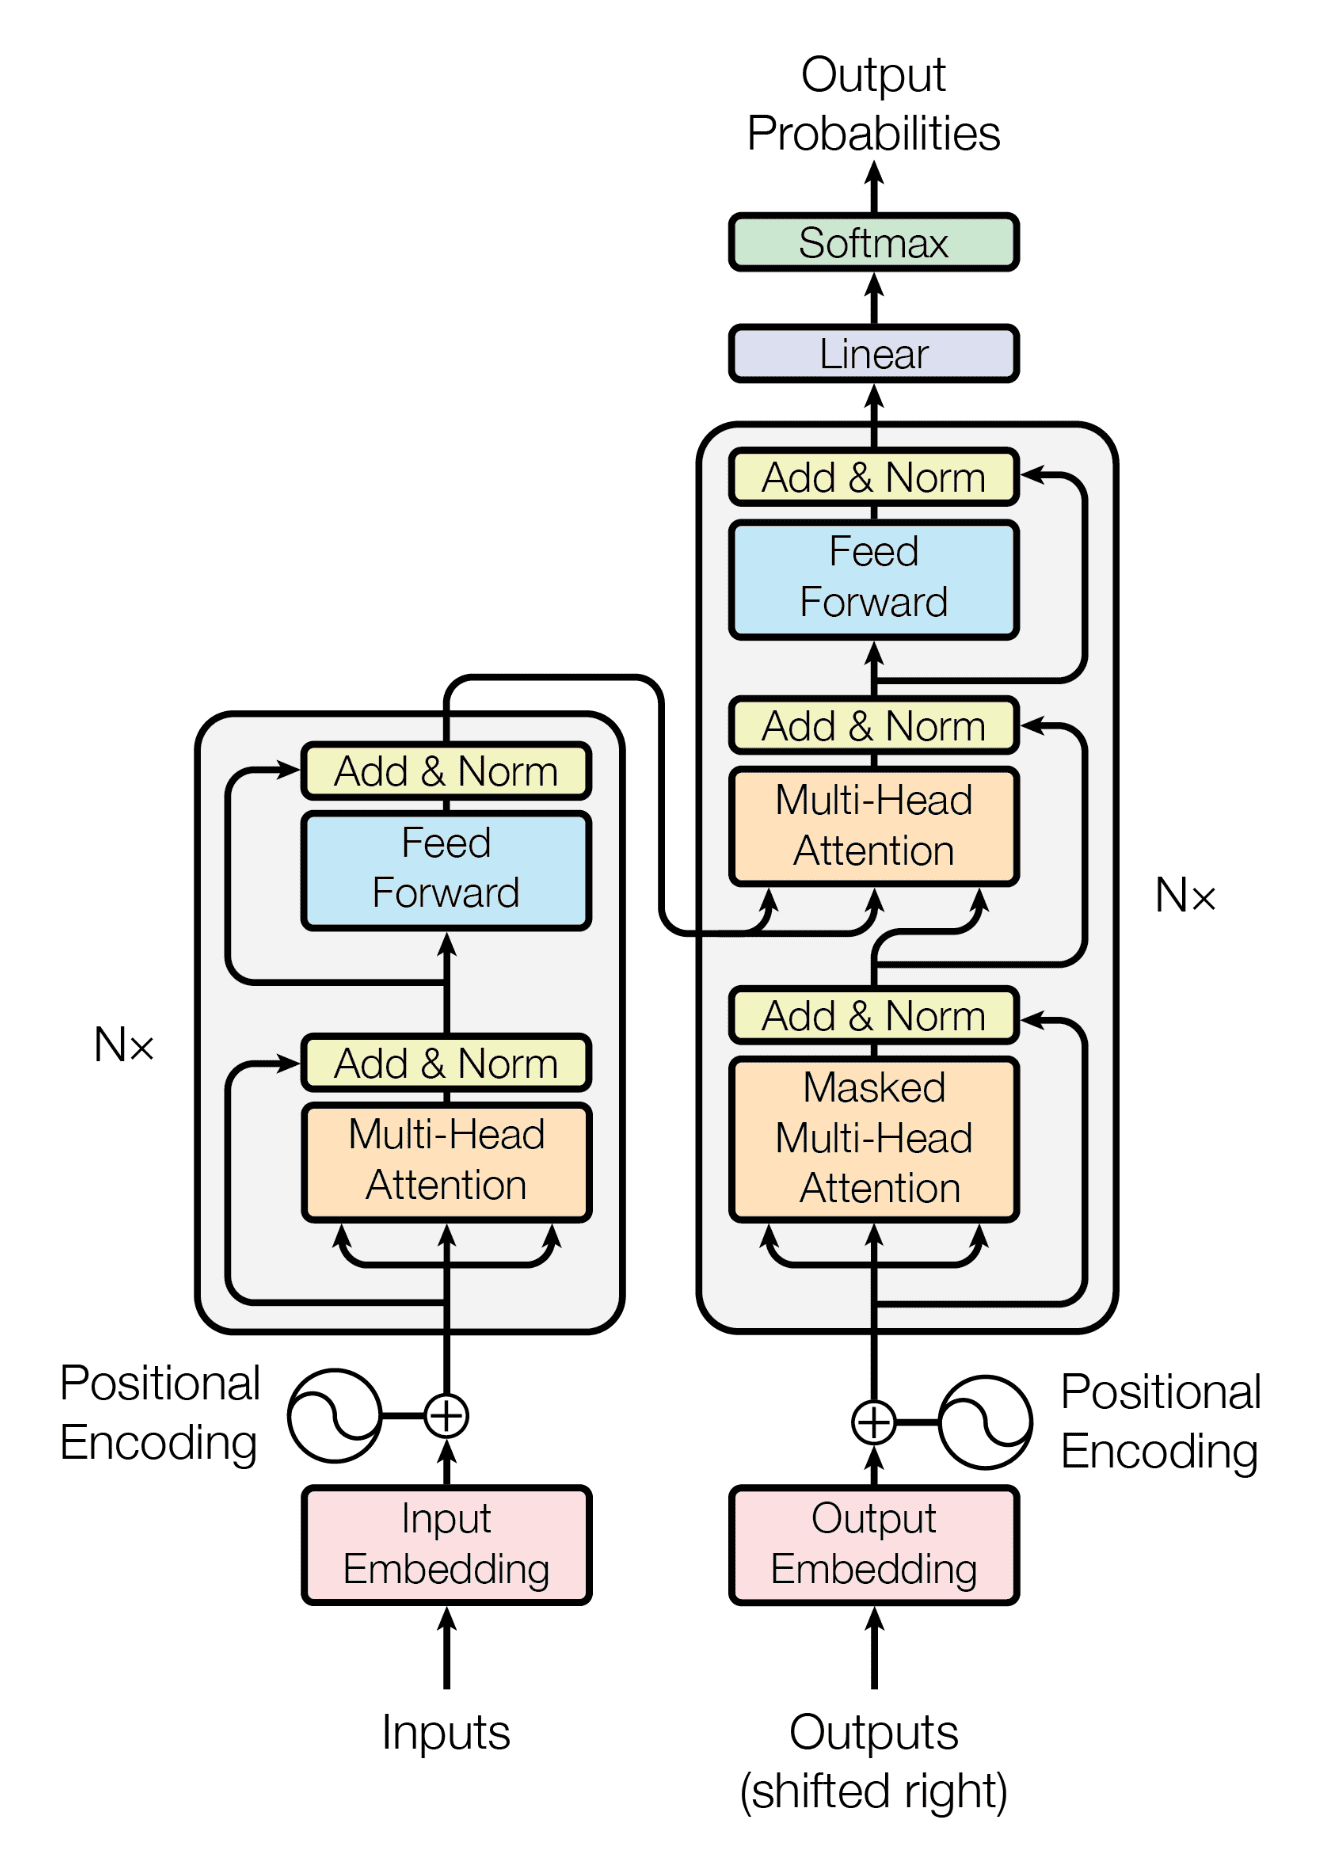
\includegraphics[width=\linewidth]{figures/transformer_architecture.png}


\section{Large Language Model}

Large Language Model (LLM) bezeichnet ein Language Model, das auf vielen Parametern trainiert wurde. 
Dabei versteht man unter Language Model ein Sprachmodell in Anlehnung an die natürlicher Sprache.
Die meisten modernen LLMs basieren auf der Transformerarchitektur, um aus einer Inputsequenz mithilfe des Encoders und des Decoders wieder eine Outputsequenz zu generieren.


Technisch gesehen ist die Funktionsweise eines LLMs nur eine Next Token Prediction.
Dabei wird nach Verarbeitung der Input Sequenz eine Wahrscheinlichkeit des Auftretens verschiedener Token ermittelt.
Das LLM generiert so einfach nur Sätze, die in dem vorherigen Kontext Sinn ergeben.
Durch weitere Techniken des Finetunings können die LLMs dazu gebracht werden, auf Fragen zu antworten oder Anweisungen zu befolgen.
Die LLMs werden mit weiteren Daten trainiert, in denen zum Beispiel das Antworten auf Fragen explizit demonstriert wird.
Verschiedene LLMs können dabei auf unterschiedliche Aufgaben spezialisiert werden.
LLMs werden zum Beispiel für ChatBots, Text-Übersetzungen, Sprach-Übersetzungen, Named Entity Recognition, Sentiment Analyse oder Klassifikation eingesetzt.



\section{Chatbots}

Besonders die LLM gestützten Chatbots werden aufgrund ihrer Leistungsfähigkeit immer beliebter.
Der bekannteste Chatbot ist ChatGPT von OpenAI, welcher auf einem LLM beruht, das auf ca. 175 Milliarden Parameter trainiert wurde. [https://www.ankursnewsletter.com/p/gpt-4-gpt-3-and-gpt-35-turbo-a-review]
Weitere bekannte ChatBots sind Google Gemini, die Claude Chatbots von der Firma Anthropic oder Pi von Inflection AI.

Neben den bekannten kommerziellen Chatbots, die von großen Tech Firmen entwickelt werden, entstehen immer mehr Open-Source Modelle, die zwar (noch) nicht so leistungsstark sind, aber auf eigener Hardware lokal laufen können.
Bekannte Open-Source Modelle sind zum Beispiel Gemma von Google, LLama 2 von Meta oder Mixtral von Mistral AI.
Diese Open-Source Modelle sind meist wesentlich kleiner als die kommerziellen Chatbots und können somit auf lokaler Consumer Hardware laufen.
Typische Größen für Open-Source LLMs sind 7 Milliarden-, 13 Milliarden-, 30 Milliarden- und 70 Milliarden-Parameter, das neueste Google Gemma Modell hat sogar eine Variante mit nur 2 Milliarden-Parametern.


Die Vorteile eines selbst gehosteten LLMs sind vor allem die Datensicherheit und die Möglichkeit, die Modelle auf die eigenen Aufgaben zu spezialisieren durch die Technik des Fine-Tunings.
Dabei werden Basis-Chatbots wie LLama 2 auf weiteren spezifischen Beispielen trainiert, um bestimmte Fähigkeiten des Models zu verbessern.

In dieser Arbeit wird aufgrund von fehlenden konsistenten Hardwareressourcen und zugunsten der Schnelligkeit noch auf das kommerzielle Produkt ChatGPT zugegriffen, um eigene Datenverarbeitungen durchzuführen.
In Zukunft könnte aufgrund der immer besseren und kleineren Open-Source LLMs diese Funktionalität auch auf selbstgehostete LLMs verlagert werden.

\section{Hugging Face}

Da es mittlerweile eine Vielzahl unterschiedlicher LLMs gibt, die alle verschiedene spezielle Aufgaben besitzen und in bestimmten Aspekten jeweils Vor- und Nachteile aufweisen, ist es sinnvoll, diese untereinander vergleichen zu können.
Eine solche Vergleichsmöglichkeit bietet die Plattform Hugging Face, auf der über 500.000 Machine Learning Modelle, davon mehr als 200.000 Transformer gehostet werden.

In der Kategorie "Question Answering", gibt es über 1300 Einträge und in der Kategorie "Sentence Similarity" ca. 3000.
In beiden Kategorien existieren Embedding Modelle.
Die einzelnen Modelle können kostenlos heruntergeladen werden, sie sind ausführlich dokumentiert und sie sind untereinander mithilfe einer Punkteabgabe auf verschiedenen Kontroll-Datensätzen vergleichbar.
Durch Leaderboards können die besten Modelle bestimmt werden.

\section{Massive Text Embedding Benchmark}

Hier wird beispielhaft das Massive Text Embedding Benchmark (MTEB) Leaderbord https://huggingface.co/spaces/mteb/leaderboard betrachtet.

Auf diesem Leaderboard werden Embedding Modelle auf 58 verschiedenen Datenbeständen in 112 Sprachen evaluiert.
Die Datenbestände sind dabei in acht verschiedene Aufgabenkategorien geteilt:
Bitext Mining, Classification, Clustering, Pair Classification, Reranking, Retrieval, Semantic Textual Similarity und Summarization.

Für diese Arbeit sind vor allem die einzelnen Aufgabenbereiche Retrieval und Reranking interessant. Im Bereich Retrieval besteht die Aufgabe, aus einer großen Menge an Daten, relevante Dokumente zu einem bestimmten Thema zu finden.
Bei der Reranking Aufgabe gilt es, eine Liste an potentiell passenden Dokumenten nach Wichtigkeit zu sortieren.
Im Aufgabenbereich Retrieval werden die einzelnen Embeddings auf 15 verschiedene Datenbeständen evaluiert.

\cite{muennighoff2023}

Leider ist eine Evaluation auf deutscher Sprache noch nicht möglich, da zu wenig Datenbestände zur Verfügung stehen. 
In Zukunft, wenn mehr Datenbestände für die deutsche Sprache entwickelt wurden, wird die Evaluation um eine deutsche Kategorie erweitert. \cite{muennighoff2023a}
In Kapitel \autoref{ch:experiments} wird versucht die besten Embedding Modelle für die Retrieval Aufgabe des Podcast-Generators zu ermitteln.


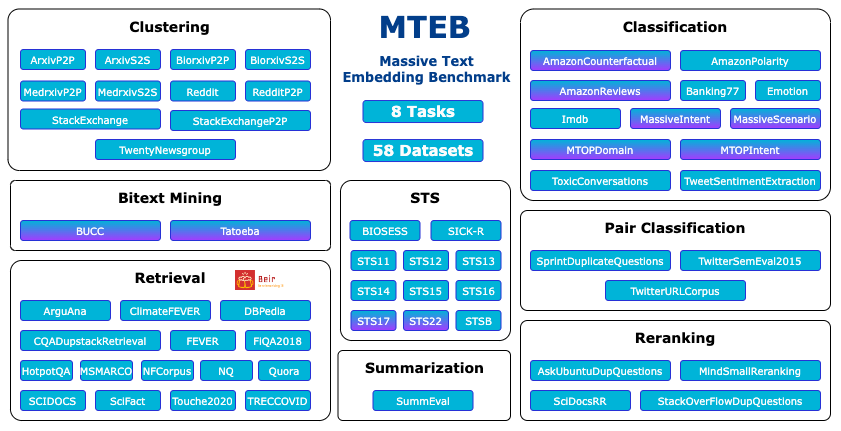
\includegraphics[width=\linewidth]{figures/mteb.png}



